% \documentclass[conference]{IEEEtran}
% \documentclass[letterpaper, 10 pt, conference]{ieeeconf}
\documentclass[conference]{IEEEtran}
\usepackage{amsmath,amssymb,amsfonts,bm}
\usepackage{graphicx}
\usepackage{booktabs}
\usepackage{array}
\usepackage{multirow}
\usepackage{xcolor}
\usepackage{cite}
\usepackage{url}

\usepackage{graphics}
\usepackage{epsfig}
\usepackage{times}
\usepackage{amsmath}
\usepackage{amssymb}
\usepackage{colortbl}
\usepackage{tabularx}
\usepackage{amsfonts}
\usepackage{booktabs}
\usepackage{makecell}
\usepackage{soul}
\usepackage{xcolor}
\usepackage{bm}
\usepackage{duckuments}
\usepackage{lipsum}
\usepackage{kotex}
\usepackage{cite}
\usepackage{hyperref}

\hypersetup{
    colorlinks=true,
    citecolor=blue,
    linkcolor=blue,
    urlcolor=blue
}

\title{
Nonlinear Trajectory Optimization and Stabilization for Swing-Up of a Double Inverted Pendulum on a Cart
}

\author{
\IEEEauthorblockN{JunYoung Kim}
\IEEEauthorblockA{Department of Mechanical and Aerospace Engineering\\
MAE589: Advanced Robotics Course Project Report}
}

\begin{document}
\maketitle
\thispagestyle{empty}
\pagestyle{empty}

\begin{abstract}
This paper presents a nonlinear optimal-control approach for swing-up and stabilization of a double inverted pendulum on a cart. The problem is challenging because the system is strongly nonlinear and underactuated. The proposed method first computes a finite-horizon trajectory using direct nonlinear trajectory optimization over the full manipulator dynamics. A local linear-quadratic regulator (LQR) is then activated near the upright configuration to stabilize the terminal equilibrium after the swing-up maneuver. The same trajectory-optimization framework is extended to obstacle-aware planning by adding a smooth workspace penalty over sampled points on the cart and links. Simulation results show that the nominal planner generates a dynamically feasible swing-up trajectory, while the obstacle-aware planner produces collision-avoiding motions that are subsequently stabilized by LQR.
\end{abstract}

\section{Introduction}
The double inverted pendulum on a cart is a representative benchmark for nonlinear, underactuated control. A single cart force must move the cart and simultaneously transfer energy into two pendulum links. As a result, the swing-up task cannot be solved by independently commanding each coordinate. The controller must exploit inertial coupling, generate large transient motion, and arrive close enough to the upright equilibrium for local stabilization.

The difficulty is amplified by the nonlinear behavior of the mechanism. Even without actuation, a double-pendulum system can produce sensitive and visually complex transient motion. Small changes in phase or angular velocity may lead to very different tip paths, which makes global swing-up fundamentally different from small-signal regulation around the upright equilibrium. Typical approaches therefore separate the problem into two parts: a global motion-generation phase that uses nonlinear planning or energy-based control, followed by a local stabilizing controller near the desired equilibrium.

This paper combines nonlinear trajectory optimization, obstacle-aware trajectory shaping, and LQR terminal stabilization. The trajectory optimizer is responsible for discovering a dynamically feasible swing-up motion under the full nonlinear model. The LQR controller then holds the cart and links near the target after the planned maneuver reaches the upright neighborhood.

\section{Preliminaries and Problem Statement}
\subsection{Finite-Horizon Optimal Control}
Consider a nonlinear control system
\begin{equation}
\dot{\bm{x}}(t)=\bm{f}(\bm{x}(t),u(t)),
\end{equation}
where $\bm{x}(t)\in\mathbb{R}^{n}$ is the state and $u(t)\in\mathcal{U}$ is the control input. A finite-horizon optimal-control problem seeks a state trajectory and an input trajectory that minimize
\begin{align}
\min_{\bm{x}(\cdot),u(\cdot)} \quad &
\int_0^T \ell(\bm{x}(t),u(t),t)\,dt+\phi(\bm{x}(T)) \\
\text{s.t.}\quad &
\dot{\bm{x}}(t)=\bm{f}(\bm{x}(t),u(t)), \\
& \bm{x}(0)=\bm{x}_{\mathrm{init}}, \\
& u(t)\in\mathcal{U}.
\label{eq:continuousocp}
\end{align}
Here $\ell$ is the running cost, which penalizes behavior along the trajectory, and $\phi$ is the terminal cost, which penalizes the final state. In this project, $\mathcal{U}$ is the allowable interval of horizontal cart forces, $\bm{x}_{\mathrm{init}}$ is a configuration near the downward hanging pose, and the desired terminal state is the upright equilibrium at a specified cart position.

\begin{figure*}[t]
\centering
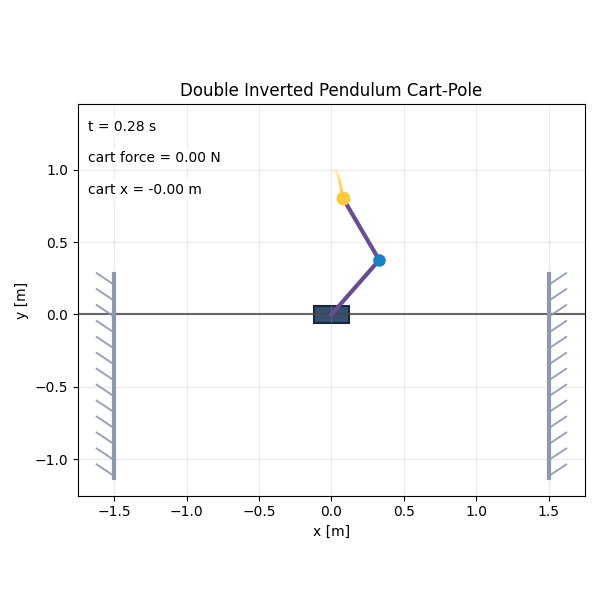
\includegraphics[width=0.325\linewidth]{figures/chaotic/Figure_0.png}
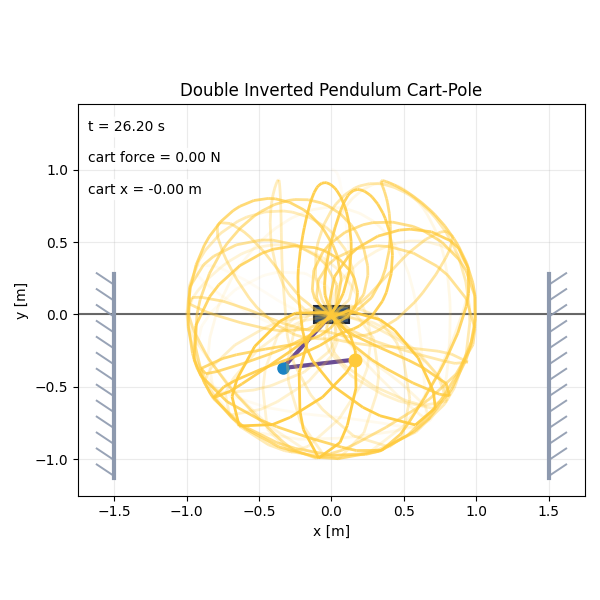
\includegraphics[width=0.325\linewidth]{figures/chaotic/Figure_2.png}
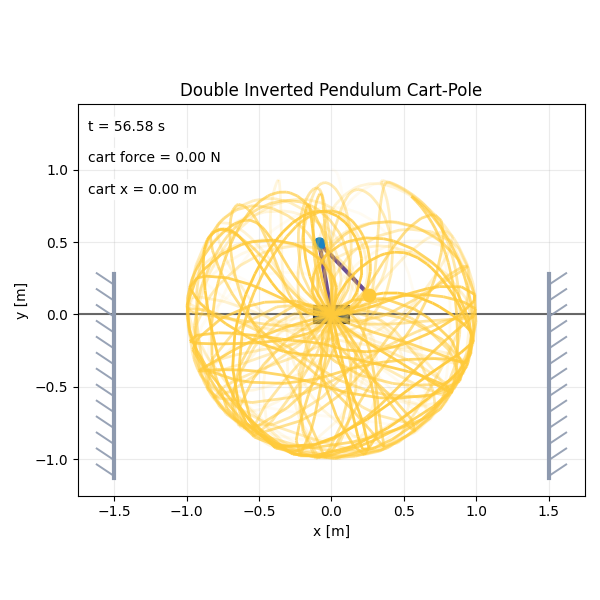
\includegraphics[width=0.325\linewidth]{figures/chaotic/Figure_4.png}
\vspace{-15pt}
\caption{Representative passive motion of the cart--double-pendulum under zero input. The yellow curve is the accumulated end-tip path, shown at three instants from the same rollout. Even without active control, the coupled nonlinear dynamics produce large-amplitude motion and complicated transient traces. This behavior motivates a global nonlinear planning method for swing-up rather than relying only on a local controller designed around the upright equilibrium.}
\label{fig:chaotic}
\end{figure*}

\subsection{Underactuation and Nonlinear Behavior}
The cart--double-pendulum has three generalized coordinates but only one actuator. This means the system is underactuated: the cart coordinate is directly forced, but the two angular coordinates are influenced indirectly through gravity and inertial coupling. Underactuation makes the problem a planning task rather than a direct tracking task, because the desired angular motion must be created by the cart motion.

The nonlinear behavior of the system is illustrated in Fig.~\ref{fig:chaotic}. The figure shows representative passive motion with the end-tip trace retained over time. This behavior motivates why local linear control alone is not suitable for the full swing-up problem. A local controller can stabilize small deviations near an equilibrium, but it does not by itself provide the large-amplitude motion needed to move from the hanging configuration to the upright configuration. Therefore, the method used here first solves a nonlinear finite-horizon planning problem and then switches to a local stabilizer only near the end of the maneuver.

\section{System Model}
\subsection{Coordinates, State, and Control}
Let the generalized coordinate vector be
\begin{equation}
\bm{q}=\begin{bmatrix}x&\theta_1&\theta_2\end{bmatrix}^{\top},
\end{equation}
where $x$ is the horizontal cart position and $\theta_1,\theta_2$ are the first and second link angles measured from the upright vertical direction. With this convention, $\theta_1=\theta_2=0$ corresponds to the upright pose and $\theta_1=\theta_2=\pi$ corresponds to the downward hanging pose.

The state vector is
\begin{equation}
\bm{x}
=
\begin{bmatrix}
x & \theta_1 & \theta_2 & \dot{x} & \dot{\theta}_1 & \dot{\theta}_2
\end{bmatrix}^{\top},
\end{equation}
and the scalar control input $u$ is the horizontal force applied to the cart. The target state is denoted by $\bm{x}^{\star}$ and corresponds to the upright link angles, zero velocities, and the desired cart location.

\subsection{Kinematic Convention}
The cart position is
\begin{equation}
\bm{p}_c=\begin{bmatrix}x\\0\end{bmatrix}.
\end{equation}
Using the global-angle convention above, the first joint position and end-tip position are
\begin{align}
\bm{p}_1
&=
\bm{p}_c+
\begin{bmatrix}
l_1\sin\theta_1\\
l_1\cos\theta_1
\end{bmatrix},\\
\bm{p}_2
&=
\bm{p}_1+
\begin{bmatrix}
l_2\sin\theta_2\\
l_2\cos\theta_2
\end{bmatrix},
\end{align}
where $l_1$ and $l_2$ are the two link lengths. This convention is important because the angular coordinates are periodic. Consequently, the trajectory objective uses periodic angle penalties instead of treating angular error as an ordinary Euclidean difference.

\subsection{Dynamic Model}
The equations of motion are written in manipulator form as
\begin{equation}
\bm{M}(\bm{q})\ddot{\bm{q}}
=
\bm{\tau}(\bm{q},\dot{\bm{q}},u),
\label{eq:manip}
\end{equation}
where $\bm{M}(\bm{q})$ is the mass matrix and $\bm{\tau}$ collects the generalized forces from control, gravity, damping, and velocity-dependent coupling. The mass matrix is
\begin{equation}
\resizebox{0.98\columnwidth}{!}{$
\displaystyle
\bm{M}(\bm{q}) =
\begin{bmatrix}
m_0 + m_1 + m_2 & (m_1+m_2)l_1\cos\theta_1 & m_2l_2\cos\theta_2 \\
(m_1+m_2)l_1\cos\theta_1 & (m_1+m_2)l_1^2 & m_2l_1l_2\cos(\theta_1-\theta_2) \\
m_2l_2\cos\theta_2 & m_2l_1l_2\cos(\theta_1-\theta_2) & m_2l_2^2
\end{bmatrix}.
$}
\label{eq:massmatrix}
\end{equation}
The generalized-force vector is
\begin{equation}
\resizebox{0.98\columnwidth}{!}{$
\displaystyle
\bm{\tau} =
\begin{bmatrix}
u - d_x \dot{x} + (m_1+m_2)l_1\sin\theta_1 \dot{\theta}_1^2 + m_2l_2\sin\theta_2 \dot{\theta}_2^2 \\
-d_1 \dot{\theta}_1 - m_2l_1l_2\sin(\theta_1-\theta_2)\dot{\theta}_2^2 + (m_1+m_2)gl_1\sin\theta_1 \\
-d_2 \dot{\theta}_2 + m_2l_1l_2\sin(\theta_1-\theta_2)\dot{\theta}_1^2 + m_2gl_2\sin\theta_2
\end{bmatrix}.
$}
\label{eq:generalizedforce}
\end{equation}
The off-diagonal terms in \eqref{eq:massmatrix} encode the coupling between the cart and the two links. This coupling is what allows the single cart input to generate angular swing-up motion, but it also makes the resulting trajectory highly nonlinear.

Solving \eqref{eq:manip} for $\ddot{\bm{q}}$ gives the first-order state equation
\begin{equation}
\dot{\bm{x}}
=
\bm{f}(\bm{x},u)
=
\begin{bmatrix}
\dot{x} & \dot{\theta}_1 & \dot{\theta}_2 &
\ddot{x} & \ddot{\theta}_1 & \ddot{\theta}_2
\end{bmatrix}^{\top}.
\end{equation}

\subsection{Task Definition}
The task is to move the system from a near-downward initial configuration to an upright target configuration at a target cart position. The desired final state is
\begin{equation}
\bm{x}^{\star}
=
\begin{bmatrix}
x_g&0&0&0&0&0
\end{bmatrix}^{\top},
\end{equation}
where $x_g$ is the goal cart position. The planner is not given a stabilizing feedback law during the nonlinear optimization. Instead, it computes a nominal swing-up trajectory over a finite horizon, and a separate local feedback controller is used once the trajectory enters a terminal neighborhood of the upright target.

% \section{Optimal-Control Interpretation}
% \subsection{Pontryagin Minimum Principle}
% Before discretizing the problem, it is useful to interpret the swing-up task as a continuous-time optimal-control problem. Let $L(\bm{x},u,t)$ be the running cost and let $\phi(\bm{x}(T))$ be the terminal cost. Following the sign convention used in class, define the Hamiltonian
% \begin{equation}
% H(\bm{x},u,\bm{p},t)
% =
% \bm{p}^{\top}\bm{f}(\bm{x},u)-L(\bm{x},u,t),
% \label{eq:hamiltonian}
% \end{equation}
% where $\bm{p}(t)\in\mathbb{R}^{6}$ is the costate vector. The costate is the Lagrange multiplier associated with the differential constraint $\dot{\bm{x}}=\bm{f}(\bm{x},u)$. Equivalently, the constrained objective can be written as
% \begin{equation}
% \bar{J}
% =
% \phi(\bm{x}(T))
% +
% \int_0^T
% \left[
% L(\bm{x},u,t)
% +
% \bm{p}^{\top}\big(\bm{f}(\bm{x},u)-\dot{\bm{x}}\big)
% \right]dt .
% \end{equation}
% The first-order necessary conditions from Pontryagin's minimum principle (PMP) are
% \begin{align}
% \dot{\bm{x}}^{*}(t)
% &=
% \frac{\partial H}{\partial \bm{p}}
% \big(\bm{x}^{*}(t),u^{*}(t),\bm{p}^{*}(t),t\big),\\
% \dot{\bm{p}}^{*}(t)
% &=
% -
% \frac{\partial H}{\partial \bm{x}}
% \big(\bm{x}^{*}(t),u^{*}(t),\bm{p}^{*}(t),t\big),\\
% u^{*}(t)
% &\in
% \arg\max_{u\in\mathcal{U}}
% H\big(\bm{x}^{*}(t),u,\bm{p}^{*}(t),t\big),\\
% \bm{p}^{*}(T)
% &=
% -\nabla_{\bm{x}}\phi(\bm{x}^{*}(T)).
% \end{align}
% These equations show that the optimal trajectory must satisfy both the physical dynamics and an adjoint sensitivity equation. For the present system, directly solving this two-point boundary-value problem is inconvenient, so the project uses direct trajectory optimization instead.

% \subsection{Hamilton--Jacobi--Bellman Viewpoint}
% The Hamilton--Jacobi--Bellman (HJB) viewpoint describes the same problem through a value function rather than a single extremal trajectory. Define
% \begin{equation}
% V(\bm{x},t)
% =
% \min_{u(\cdot)}
% \left[
% \phi(\bm{x}(T))
% +
% \int_t^T L(\bm{x}(\tau),u(\tau),\tau)\,d\tau
% \right],
% \label{eq:value_function}
% \end{equation}
% where $V(\bm{x},t)$ is the minimum cost-to-go from state $\bm{x}$ at time $t$. Bellman's principle gives
% \begin{equation}
% \frac{\partial V}{\partial t}
% =
% \sup_{u\in\mathcal{U}}
% \left[
% -L(\bm{x},u,t)
% -
% \nabla_{\bm{x}}V(\bm{x},t)^{\top}\bm{f}(\bm{x},u)
% \right],
% \label{eq:hjb}
% \end{equation}
% with terminal boundary condition $V(\bm{x},T)=\phi(\bm{x})$. Under the Hamiltonian convention in \eqref{eq:hamiltonian}, the PMP costate is related to the value gradient by
% \begin{equation}
% \bm{p}(t)=-\nabla_{\bm{x}}V(\bm{x}(t),t).
% \end{equation}
% Thus PMP and HJB provide complementary interpretations: PMP gives necessary conditions along an optimal path, while HJB describes the optimal cost-to-go over the state space. Computing the full HJB solution is not practical for this six-state nonlinear system, but the viewpoint explains why a local quadratic value approximation near the upright equilibrium naturally leads to an LQR stabilizer.

\section{Discrete Trajectory Optimization and Stabilization}
\subsection{Reference Curve}
A smooth reference curve is used to initialize the nonlinear program and to give the stage cost a nominal direction. For the normalized time index
\begin{equation}
\tau_k=\frac{k}{N},\qquad k=0,\ldots,N,
\end{equation}
the cubic smoothstep function is
\begin{equation}
s(\tau)=3\tau^2-2\tau^3 .
\end{equation}
The reference cart position and link angles interpolate from the initial state to the target state according to this scalar profile. The velocity components of the reference are set to zero. This reference is not assumed to be dynamically feasible; it only provides an initial guess and a soft shaping signal for the optimizer.

For each reference state, a nominal feedforward force is computed by choosing the input that gives the smallest generalized acceleration magnitude within the actuator range. This force sequence is used only as a regularization reference in the objective.

\subsection{Overall Nonlinear Program}
The finite-dimensional problem is the central object of the method. The optimizer searches over all discrete states and inputs at once:
\begin{align}
\min_{\bm{X},\bm{U}} \quad &
\sum_{k=0}^{N-1}\ell_k(\bm{x}_k,u_k)
+
\phi(\bm{x}_N)
+
J_{\mathrm{obs}}(\bm{X})
\label{eq:discrete_nlp}\\
\text{s.t.}\quad &
\bm{x}_0=\bm{x}_{\mathrm{init}},\\
& \bm{x}_{k+1}=\Phi_{\mathrm{RK4}}(\bm{x}_k,u_k),
\quad k=0,\ldots,N-1,\\
& -u_{\max}\leq u_k\leq u_{\max},
\quad k=0,\ldots,N-1 .
\label{eq:force_constraints}
\end{align}
Here $\ell_k$ is the running cost, $\phi$ is the terminal cost, and $J_{\mathrm{obs}}$ is an optional obstacle penalty. When no obstacles are present, $J_{\mathrm{obs}}$ is set to zero.

The discrete state sequence $\bm{X}=[\bm{x}_0,\bm{x}_1,\ldots,\bm{x}_N]$ and input sequence $\bm{U}=[u_0,u_1,\ldots,u_{N-1}]$ are the decision variables. The equality constraint in \eqref{eq:discrete_nlp} is the direct-transcription constraint that enforces the nonlinear dynamics between adjacent nodes. In the implementation, $\Phi_{\mathrm{RK4}}$ denotes one fourth-order Runge--Kutta integration step with time step $\Delta t$. Thus, the optimizer is not simply interpolating between the initial and terminal states; it must choose a trajectory that is consistent with the simulated nonlinear dynamics. The bound in \eqref{eq:force_constraints} enforces the allowable cart-force range at every input node.

\subsection{Running Cost}
The trajectory optimizer balances reference shaping, angular alignment, control effort, and input smoothness. The path cost at node $k$ is written generically as
\begin{align}
\ell_k
&=
\|\bm{x}_k-\bm{x}_k^{\mathrm{ref}}\|_{\bm{Q}_{\mathrm{path}}}^{2}
+
w_{\theta,p}\Gamma_k
\nonumber\\
&\quad+
w_u(u_k-u_k^{\mathrm{ref}})^2
+
w_{\Delta u}(u_k-u_{k-1})^2 ,
\label{eq:pathcost}
\end{align}
where $u_k^{\mathrm{ref}}$ is the nominal input reference, and $\Gamma_k$ is the periodic angular tracking penalty
\begin{equation}
\Gamma_k
=
1-\cos(\theta_{1,k}-\theta_{1,k}^{\mathrm{ref}})
+
1-\cos(\theta_{2,k}-\theta_{2,k}^{\mathrm{ref}}).
\end{equation}
The periodic penalty avoids artificial discontinuities when angular differences cross a $2\pi$ boundary. This is important because the swing-up motion can rotate through large angles even though the desired terminal angles are near zero.

\subsection{Terminal Cost}
The terminal cost penalizes the final deviation from the desired upright state:
\begin{equation}
\phi(\bm{x}_N)
=
\|\bm{x}_N-\bm{x}^{\star}\|_{\bm{Q}_{\mathrm{term}}}^{2}
+
w_{\theta,t}\Gamma_N^{\star},
\label{eq:terminal}
\end{equation}
where $\Gamma_N^{\star}$ is the same periodic angular penalty evaluated relative to the target angles. The terminal angular weight is larger than the path angular weight because reaching the upright neighborhood at the end of the horizon is more important than following the reference angles exactly during the swing-up transient.

\subsection{Obstacle-Aware Extension}
The obstacle-aware extension keeps the same nonlinear program in \eqref{eq:discrete_nlp} and adds a smooth workspace penalty. The key idea is to evaluate clearance for the physical body of the mechanism, not only for the cart position or the pendulum tip. At time step $k$, let
\begin{equation}
\mathcal{P}(\bm{x}_k)
=
\{\bm{p}_{c,k}\}
\cup
\{\bm{p}^{(1)}_{j,k}\}_{j=1}^{n_s}
\cup
\{\bm{p}^{(2)}_{j,k}\}_{j=1}^{n_s}
\end{equation}
be the finite set of sampled body points, where $\bm{p}_{c,k}$ is the cart point and $\bm{p}^{(1)}_{j,k}$ and $\bm{p}^{(2)}_{j,k}$ are points sampled along the first and second links. Let $\mathcal{O}$ be the set of rectangular obstacles. For a sampled point $\bm{p}$ and obstacle $o$, define $d_o(\bm{p})$ as the signed clearance from the obstacle boundary: $d_o(\bm{p})>0$ outside the obstacle, $d_o(\bm{p})=0$ on the boundary, and $d_o(\bm{p})<0$ inside the obstacle.

The obstacle cost is
\begin{equation}
J_{\mathrm{obs}}(\bm{X})
=
\sum_{k=0}^{N}
\sum_{\bm{p}\in\mathcal{P}(\bm{x}_k)}
\sum_{o\in\mathcal{O}}
w_{\mathrm{obs}}\,
\psi\!\left(r_{\mathrm{safe}}-d_o(\bm{p})\right)^2 ,
\label{eq:obstaclecost}
\end{equation}
where $w_{\mathrm{obs}}$ is the obstacle weight, $r_{\mathrm{safe}}$ is the desired clearance margin, and $\psi(\cdot)$ is a smooth nonnegative hinge function. The argument $r_{\mathrm{safe}}-d_o(\bm{p})$ is positive only when the sampled point is inside the clearance margin of an obstacle. Therefore, points far from obstacles contribute almost no cost, while points near or inside the inflated obstacle region are penalized.

This penalty formulation is intentionally soft. It does not prove formal collision avoidance for the continuous body over all time, but it gives the nonlinear optimizer a differentiable signal that reshapes the swing-up trajectory away from obstacle regions. Sampling points along both links is essential here: without those samples, the optimizer could move the pendulum tip around an obstacle while still letting the body of a link pass through it.

\subsection{LQR Tracking and Terminal Stabilization}
The optimized trajectory is a finite-horizon plan, so it must be paired with feedback during simulation. The feedback layer has two roles. During swing-up, it tracks the optimized state and input sequence with local gains computed along the planned trajectory. Near the upright terminal neighborhood, it switches to an equilibrium LQR controller that stabilizes the final pose.

For a local linearization about a reference pair $(\bar{\bm{x}},\bar{u})$,
\begin{equation}
\delta\dot{\bm{x}}=\bm{A}\delta\bm{x}+\bm{B}\delta u,
\end{equation}
where $\delta\bm{x}=\bm{x}-\bar{\bm{x}}$, $\delta u=u-\bar{u}$, and
\begin{equation}
\bm{A}
=
\left.\frac{\partial \bm{f}}{\partial \bm{x}}\right|_{\bar{\bm{x}},\bar{u}},
\qquad
\bm{B}
=
\left.\frac{\partial \bm{f}}{\partial u}\right|_{\bar{\bm{x}},\bar{u}} .
\end{equation}
An LQR gain is obtained by minimizing the local quadratic cost
\begin{equation}
J_{\mathrm{LQR}}
=
\int_0^{\infty}
\left(
\delta\bm{x}^{\top}\bm{Q}\delta\bm{x}
+
\delta u^{\top}\bm{R}\delta u
\right)dt,
\end{equation}
where $\bm{Q}\succeq 0$ penalizes state error and $\bm{R}\succ 0$ penalizes control effort. For the terminal equilibrium $\bar{\bm{x}}=\bm{x}^{\star}$ and $\bar{u}=u^{\star}$, the continuous-time algebraic Riccati equation is
\begin{equation}
\bm{A}^{\top}\bm{P}
+
\bm{P}\bm{A}
-
\bm{P}\bm{B}\bm{R}^{-1}\bm{B}^{\top}\bm{P}
+
\bm{Q}
=
\bm{0},
\end{equation}
and the stabilizing feedback is
\begin{equation}
u
=
u^{\star}
-
\bm{K}(\bm{x}-\bm{x}^{\star}),
\qquad
\bm{K}=\bm{R}^{-1}\bm{B}^{\top}\bm{P}.
\end{equation}
The same principle is used along the planned trajectory by linearizing about the time-indexed reference states and inputs. This produces a local tracking correction around the open-loop optimized input during the swing-up phase. 

Once the state is close enough to the upright target in position, angle, and velocity, the controller switches to the terminal LQR law. Thus the trajectory optimizer handles the global nonlinear maneuver and obstacle geometry, while LQR is used only as a local feedback mechanism where the linear approximation is meaningful.

\begin{figure}[t]
\centering
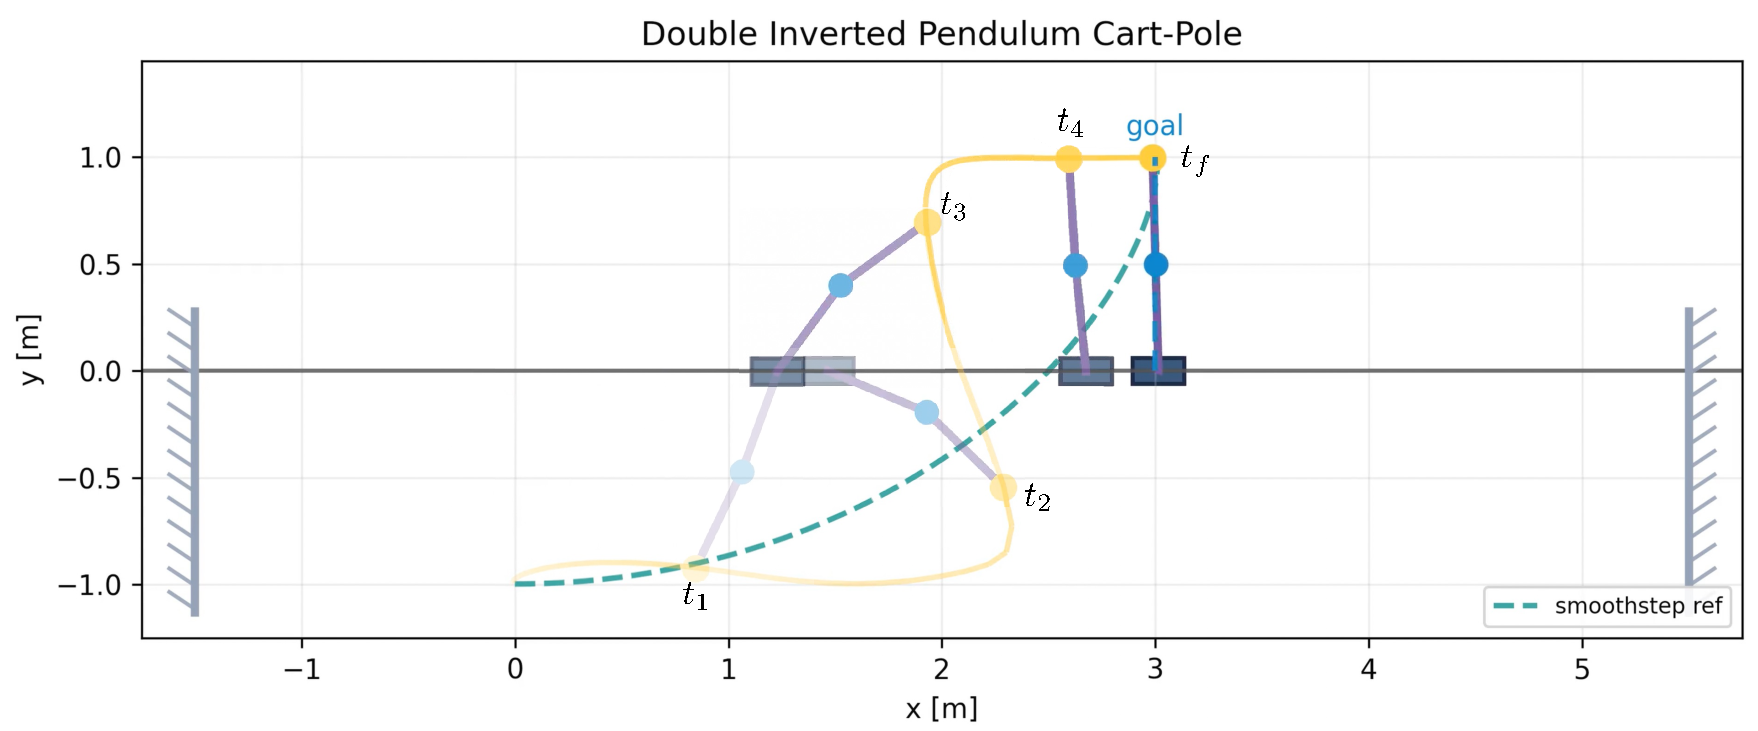
\includegraphics[width=1.0\linewidth]{figures/snapshots/snapshots_run1.pdf}
\caption{\textbf{Snapshots for Scenario 1}. The sequence shows the optimized finite-horizon motion without obstacles.}
\label{fig:trajectory_snapshot}
\end{figure}

\section{Simulation Results}
This section presents three simulation scenarios: nominal swing-up without obstacles, obstacle-aware swing-up with two obstacles, and obstacle-aware swing-up with an additional obstacle below the goal. All scenarios start near the downward configuration with $\theta_1(0)=\pi+0.08$ rad and $\theta_2(0)=\pi-0.08$ rad. The same model and optimizer are used in all cases. Model and simulation settings are summarized in Table~\ref{tab:trajparams}.

\begin{table}[b]
\caption{Simulation and Model Settings}
\label{tab:trajparams}
\centering
\begin{tabular}{l c}
\toprule
Quantity & Value \\
\midrule
Cart mass $m_0$ & $1.0$ kg \\
Link masses $m_1,m_2$ & $0.2$ kg, $0.2$ kg \\
Link lengths $l_1,l_2$ & $0.5$ m, $0.5$ m \\
Damping $(d_x,d_1,d_2)$ & $(1.0,0.1,0.01)$ \\
Force limit $u_{\max}$ & $150$ N \\
Horizon steps $N$ & $80$ \\
Time step $\Delta t$ & $0.04$ s \\
Planning horizon & $3.2$ s \\
Goal cart position $x_g$ & $3.0$ m \\
Obstacle clearance margin \qquad \qquad  \qquad \qquad & $0.24$ m \\
\bottomrule
\end{tabular}
\end{table}

\subsection*{Nominal Trajectory Optimization}
Scenario 1 demonstrates the trajectory optimizer without obstacles or terminal feedback. Figure~\ref{fig:trajectory_snapshot} shows the planned swing-up motion as a sequence of snapshots. The cart first creates a large transient motion, allowing the two links to rotate from the downward configuration toward the upright configuration. Figure~\ref{fig:trajoptplan} shows the corresponding time histories. The optimized cart trajectory departs from the smooth reference during the maneuver because the reference is dynamically infeasible; the optimizer instead finds a nonlinear motion that satisfies the constraints and reaches the upright neighborhood by the end of the horizon.

\begin{figure}[t]
\centering

\includegraphics[width=\columnwidth]{figures/trajopt_plan.pdf}
\caption{\textbf{Nominal trajectory-optimization result for Scenario 1}. Each row shows cart position, link angles, and control input over the $3.2$ s planning horizon, respectively. Solid curves are the optimized trajectory, and dashed curves are the smooth reference used for initialization and cost shaping.}
\label{fig:trajoptplan}
\end{figure}

\begin{table}[t]
\caption{Summary of the Three Reported Scenarios}
\label{tab:scenariosummary}
\centering
\begin{tabular}{l c c c}
\toprule
Case & Obstacles & LQR switch & Peak $|u|$ \\
\midrule
Scenario 1 & none & none & $77.35$ N \\
Scenario 2 & two boxes & $2.88$ s & $39.89$ N \\
Scenario 3 & three boxes & $3.20$ s & $53.18$ N \\
\bottomrule
\end{tabular}
\end{table}

\begin{figure*}[t]
\centering
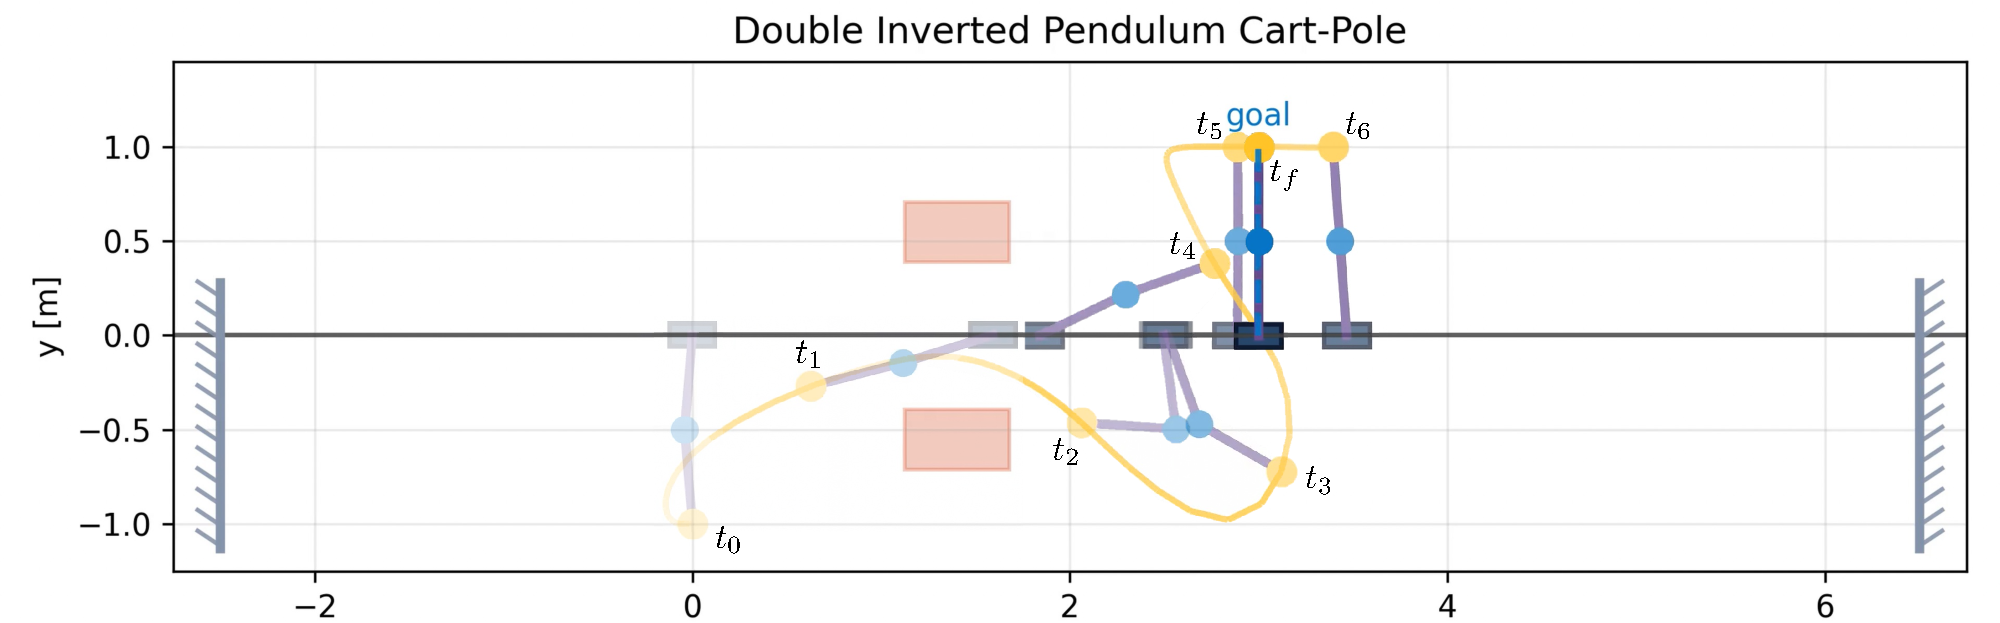
\includegraphics[width=0.82\linewidth]{figures/snapshots/snapshots_run2.pdf}
% \vspace{0.5em}
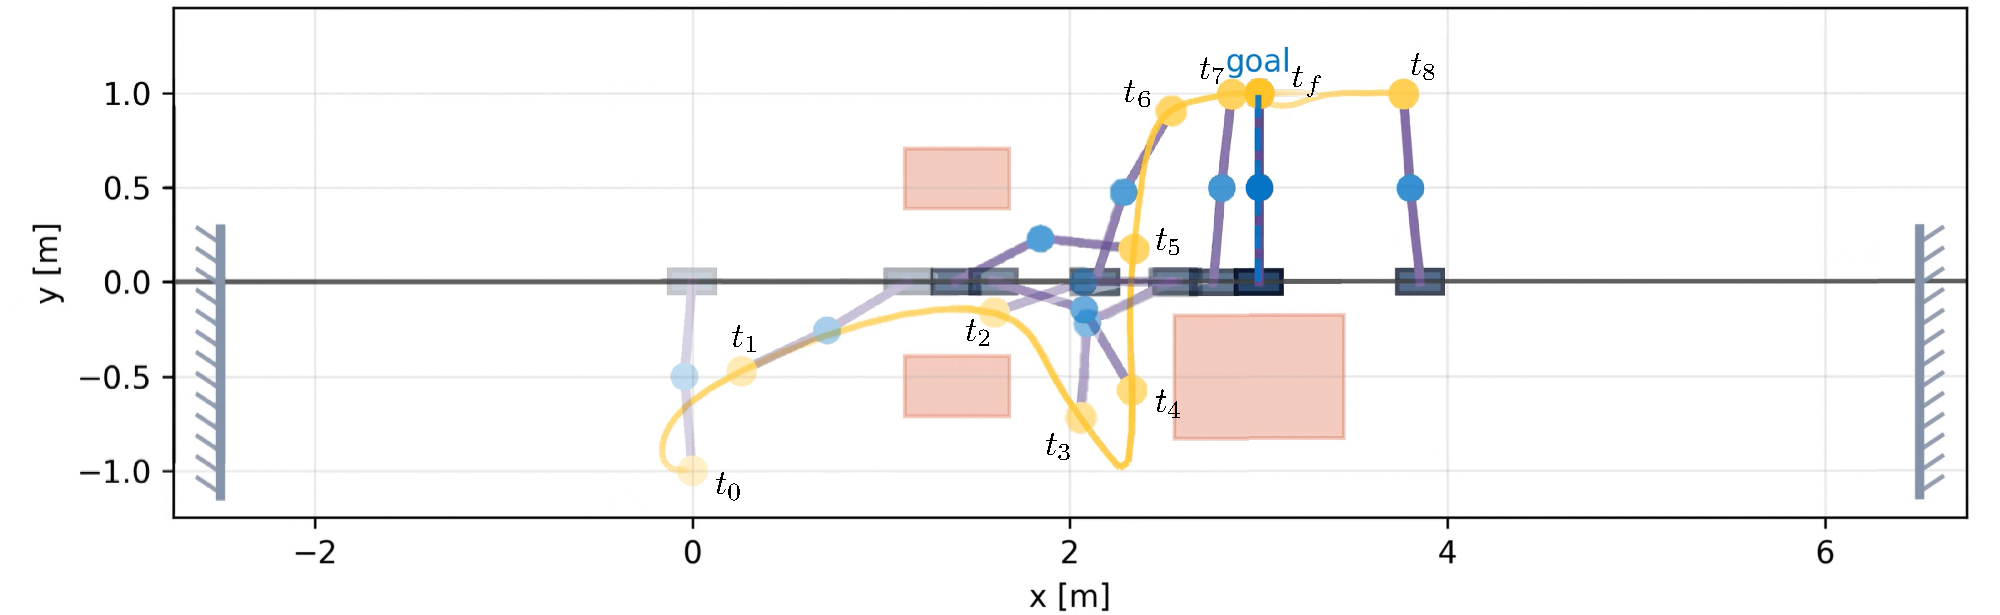
\includegraphics[width=0.82\linewidth]{figures/snapshots/snapshots_run3.pdf}
\caption{\textbf{Obstacle-aware swing-up snapshots for Scenarios 2 and 3}. The top scenario uses two rectangular obstacles, one above and one below the nominal swing-up region. The bottom scenario adds a third obstacle below the goal location, which forces a different terminal approach. In both cases, the optimizer accounts for sampled points on the cart and links, not only the end tip. The final stabilization phase is handled by the LQR controller once the trajectory enters the near-upright region.}
\label{fig:trajectory_snapshots_obstacle}
\end{figure*}

\begin{figure}[t]
\centering
% \includegraphics[width=1.0\linewidth]{figures/control_input.pdf}
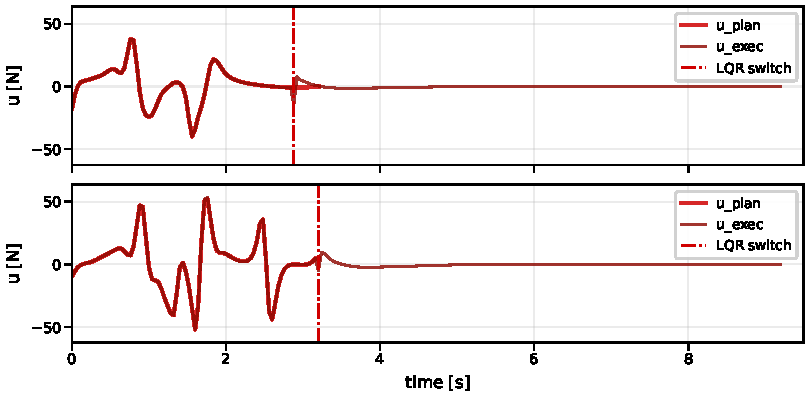
\includegraphics[width=1.0\linewidth]{figures/control_input2.pdf}
\caption{\textbf{Applied control forces for Scenarios 2 and 3}. The force remains within the actuator bound in both cases. The obstacle-aware scenarios require different input timing because the cart motion must avoid obstacles while still arriving near the upright configuration. After the LQR switch, the input decreases as the feedback controller damps the remaining motion.}
\label{fig:controlinput}
\end{figure}

\subsection*{Obstacle-Aware Swing-Up and Stabilization}
Scenarios 2 and 3 add an obstacle-avoidance cost and activate the final LQR stabilizer near the upright terminal neighborhood. Figure~\ref{fig:trajectory_snapshots_obstacle} shows both obstacle layouts. In Scenario 2, two obstacles are placed near the cart track. The optimized motion routes the links around the obstacles while still reaching a configuration suitable for stabilization. The LQR handoff occurs at $2.88$ s, after which the simulated state converges to the upright target.

Scenario 3 is more restrictive because it adds a third obstacle below the goal. This layout prevents the optimizer from simply reusing the nominal terminal approach. Instead, the optimized trajectory reaches a nearby upright configuration, and the LQR controller completes the final stabilization. The LQR handoff occurs at $3.20$ s. These results show that the obstacle penalty changes the geometry of the swing-up path while preserving the same underlying nonlinear optimization and stabilization structure.

Table~II and Fig.~5 summarize the control effort required by the reported scenarios. The nominal swing-up case reaches the upright neighborhood with a peak force of $77.35$ N, while the two obstacle-aware stabilized scenarios require peak forces of $39.89$ N and $53.18$ N, respectively. The force profiles in Fig.~5 show that both obstacle-aware cases remain within the actuator bound and that the applied input decreases after the LQR handoff as the feedback controller damps the remaining motion near the upright equilibrium.

\section{Conclusion}
This paper presented a nonlinear optimal-control pipeline for swing-up and stabilization of a double inverted pendulum on a cart. The method uses direct trajectory optimization to solve the large-amplitude underactuated swing-up problem and then switches to LQR for local stabilization near the upright equilibrium. The obstacle-aware extension shows that the same formulation can reshape the swing-up path around workspace obstacles while still using the same terminal feedback strategy. The main takeaway is that global motion generation and local stabilization should be treated as separate but connected tasks. Future work could extend this pipeline by using MPPI for feedback control, CBFs for obstacle avoidance, or PPO for learned nonlinear feedback control.

\bibliographystyle{IEEEtran}

\end{document}
